\section{Results}
\label{sec:results}

\subsection{A classical model matches a transformer on DAIGT V2 but not on HC3}

\begin{table}[!ht]
\centering
\caption{All model configurations, both datasets. Transformer rows are the deployed checkpoints, never a grid maximum, and classical rows are refits on the same split. Error rate is given beside F1 because F1 compresses at this ceiling. Bold marks the best classical and the best overall entry per dataset column. Macro F1 equals weighted F1 to four decimals in every row, so no result is produced by class skew.}
\label{tab:allmodels}
\footnotesize
\setlength{\tabcolsep}{3.5pt}
\begin{tabular}{@{}llcccc@{}}
\toprule
& & \multicolumn{2}{c}{DAIGT V2} & \multicolumn{2}{c}{HC3} \\
\cmidrule(lr){3-4}\cmidrule(lr){5-6}
Model & Rep. & F1 & err\,\% & F1 & err\,\% \\
\midrule
Naive Bayes & BoW & 0.9591 & 4.09 & 0.8713 & 12.87 \\
Naive Bayes & TF-IDF & 0.9577 & 4.23 & 0.8670 & 13.28 \\
Logistic Reg. & BoW & 0.9893 & 1.07 & \textbf{0.9551} & 4.49 \\
Logistic Reg. & TF-IDF & 0.9857 & 1.43 & 0.9365 & 6.35 \\
SVM & BoW & 0.9870 & 1.30 & 0.9475 & 5.25 \\
SVM & TF-IDF & \textbf{0.9910} & 0.90 & 0.9449 & 5.51 \\
BERT & raw & 0.9916 & 0.84 & 0.9916 & 0.84 \\
DeBERTa & raw & \textbf{0.9917} & 0.83 & \textbf{0.9972} & 0.28 \\
\bottomrule
\end{tabular}
\end{table}

Table~\ref{tab:allmodels} reports every configuration on both datasets. The two benchmarks differ in a way no single headline number reveals. On DAIGT V2 the best classical configuration, an SVM over TF-IDF at 0.9910 weighted F1, sits 0.0007 below the best transformer at 0.9917. On the same test documents the two disagree on 99 cases, 47 to 52, so the exact McNemar test returns $p=0.69$ and the paired bootstrap puts the error difference at $+0.07$ percentage points with a 95\% interval of $[-0.21, +0.34]$ that contains zero. On HC3 the same comparison is 0.9551 against 0.9972, with 484 discordant cases split 16 to 468, $p < 10^{-6}$, and an error difference of $+4.21$ points with interval $[+3.82, +4.61]$. The error-rate ratio there is sixteen to one.

\begin{figure*}[!t]
\centering

\includegraphics[width=\textwidth]{figures/fig_roc_zoom.pdf}
\caption{ROC curves for all eight model configurations, restricted to the low-false-positive region where the models actually differ. Areas under the full curve are given in the legend. On DAIGT V2 in panel (a) every configuration converges toward the corner and the classical models are close behind the transformers. On HC3 in panel (b) the two transformers separate sharply from all six classical configurations, which is the same split Table~\ref{tab:allmodels} shows and the reason a single averaged benchmark score over both corpora would hide it. Colours are colourblind-safe and each series carries a distinct dash pattern, so the ordering survives greyscale reproduction.}
\label{fig:roczoom}
\end{figure*}

Fig.~\ref{fig:roczoom} gives the corresponding ROC curves in the region that matters for a deployed detector, where false positives are expensive because they are accusations. The visual separation on HC3 and the absence of it on DAIGT V2 restate the table without the compression that F1 imposes near the ceiling.

Ranking by area does not reproduce ranking by F1. On DAIGT V2, BERT attains the higher area, 0.999641 against 0.999144, while DeBERTa attains the higher F1. Neither ordering is real, since the two models disagree on only 75 documents, 37 to 38, at $p=1.00$. On HC3 the pair separates cleanly at $p < 10^{-6}$. We report both measures for this reason, and we would draw no conclusion from either ordering on DAIGT V2.

\begin{figure*}[!t]
\centering

\includegraphics[width=\textwidth]{figures/fig_roc.pdf}
\caption{The same eight configurations over the full ROC range. At this scale every curve is close to the corner on both corpora, which is what a headline accuracy figure reports and what motivates the low-false-positive view in Fig.~\ref{fig:roczoom}. The figure is included because the compressed view is the one most often published, and the contrast between the two panels is the point.}
\label{fig:roc}
\end{figure*}

Fig.~\ref{fig:roc} shows the same curves unzoomed. The comparison between it and Fig.~\ref{fig:roczoom} is itself a small methodological observation, since at full scale the two corpora look alike and every model looks solved.

\FloatBarrier
\subsection{Error structure is one-directional on neither corpus}

\begin{figure*}[!t]
\centering

\includegraphics[width=\textwidth]{figures/fig_confusion.pdf}
\caption{Confusion matrices for the deployed BERT and DeBERTa checkpoints on both corpora, counts normalised within each true-label row. Errors are close to symmetric between the two directions on all four panels, so neither model is trading one error type for the other at its operating point. This matters for reading Section~\ref{sec:labelfree}, where the same models under perturbation produce a sharply one-directional matrix instead.}
\label{fig:confusion}
\end{figure*}

Fig.~\ref{fig:confusion} shows where the remaining errors fall. On unperturbed test data the four deployed checkpoints distribute their errors roughly evenly between calling a human document machine-generated and the reverse. That symmetry is the baseline against which the perturbation result in Section~\ref{sec:labelfree} should be read, because the collapse reported there is not a uniform loss of accuracy but a wholesale movement of one class into the other.

\FloatBarrier
\subsection{The DAIGT V2 tie is a text budget, not an architecture result}
\label{sec:budget}

\begin{table}[!ht]
\centering
\caption{Classical models refitted on the exact character span each transformer's own tokeniser retained, so both sides read the same text. The window is defined by offset mapping with no decode round-trip. Held to one budget the transformer leads on both corpora, and the DAIGT V2 tie in Table~\ref{tab:allmodels} disappears. The two tokenisers define nearly the same window and return the same conclusion.}
\label{tab:budget}
\footnotesize
\setlength{\tabcolsep}{3.5pt}
\begin{tabular}{@{}llcccc@{}}
\toprule
& & chars & \multicolumn{2}{c}{best classical err\,\%} & transf. \\
\cmidrule(lr){4-5}
Data & Window & kept & full text & 128-tok & err\,\% \\
\midrule
DAIGT V2 & BERT & 0.335 & 0.90 & 2.10 & 0.84 \\
DAIGT V2 & DeBERTa & 0.341 & 0.90 & 2.09 & 0.83 \\
HC3 & BERT & 0.746 & 4.49 & 5.66 & 0.84 \\
HC3 & DeBERTa & 0.756 & 4.49 & 5.72 & 0.28 \\
\bottomrule
\end{tabular}
\end{table}

That DAIGT V2 tie is not a matched comparison, and reading it as a statement about architecture would be wrong. The classical models receive the whole document while the transformers receive 128 tokens, which is 33.5\% of a mean DAIGT V2 essay against 74.6\% of a mean HC3 answer. Table~\ref{tab:budget} reports what happens when the asymmetry is removed by refitting the classical grid on the exact span each checkpoint's own tokeniser kept.

The best DAIGT V2 configuration then rises from 0.90\% to 2.10\% error against BERT's 0.84\%, a difference of 1.257 points with interval $[+0.900, +1.629]$ at $p < 10^{-6}$, and the DeBERTa window returns the same 1.257. On HC3 the gap only widens, from 4.49\% to 5.66\%. Held to one text budget the transformers lead on both corpora.

What the unmatched comparison shows is narrower and still worth stating, namely that a bag-of-words model reading a whole essay matches a transformer reading its opening. That is a claim about information access rather than about architecture, and on a corpus of long documents it is arguably the more useful of the two.

\FloatBarrier
\subsection{On HC3, orthography alone matches content alone}
\label{sec:decomp}

\begin{table}[!ht]
\centering
\caption{Surface-content decomposition. Surface-only uses 47 orthographic features and never reads a word. Content-only is unfiltered bag-of-words after punctuation, casing and non-ASCII characters are stripped. The lower block closes the document-length channel that both primary arms can otherwise read. Bold marks the better arm in each block and dataset column. The transformer is a reference point, not a matched arm.}
\label{tab:decomp}
\footnotesize
\setlength{\tabcolsep}{3.5pt}
\begin{tabular}{@{}lcccc@{}}
\toprule
& \multicolumn{2}{c}{DAIGT V2} & \multicolumn{2}{c}{HC3} \\
\cmidrule(lr){2-3}\cmidrule(lr){4-5}
Arm & F1 & err\,\% & F1 & err\,\% \\
\midrule
surface-only & 0.9214 & 7.86 & \textbf{0.9680} & \textbf{3.20} \\
content-only & \textbf{0.9901} & \textbf{0.99} & 0.9674 & 3.26 \\
full transformer & 0.9917 & 0.83 & 0.9972 & 0.28 \\
\midrule
\multicolumn{5}{@{}l}{\emph{length channel closed}}\\
length-only (3 feats) & 0.7540 & 24.59 & 0.8475 & 15.23 \\
surface-only, no length & 0.9007 & 9.93 & \textbf{0.9662} & \textbf{3.37} \\
content-only, length-norm. & \textbf{0.9906} & \textbf{0.94} & 0.9371 & 6.28 \\
\bottomrule
\end{tabular}
\end{table}

Table~\ref{tab:decomp} gives the decomposition. On HC3 the two arms are statistically indistinguishable, 3.20\% error from orthography against 3.26\% from content. They disagree on 625 documents, split 316 to 309, so the exact McNemar test returns $p=0.81$ and the paired bootstrap puts the difference at $-0.07$ percentage points with a 95\% interval of $[-0.52, +0.40]$. Forty-seven features that never read a word do as well as a bag-of-words model over the whole vocabulary.

On DAIGT V2 the same two arms separate by a factor of 7.9 in error, 7.86\% against 0.99\%, and there the separation is unambiguous, with 569 discordant documents split 44 to 525, $p < 10^{-6}$, and a difference of $+6.87$ points with interval $[+6.23, +7.52]$.

\begin{figure}[!ht]
\centering
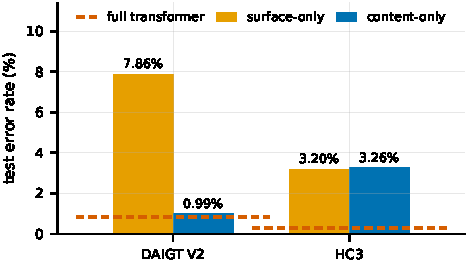
\includegraphics[width=\columnwidth]{figures/fig_decomposition.pdf}
\caption{The two primary arms and the transformer reference, per corpus. The HC3 pair is level and the DAIGT V2 pair is not, which is the paper's central observation in one view. The transformer bar is drawn in grey to mark that it is a reference point rather than a matched arm, since it differs from the other two in model family, parameter count and the amount of text it reads.}
\label{fig:decomp}
\end{figure}

Fig.~\ref{fig:decomp} shows the same three arms per corpus. Surface form is informative on both benchmarks, since DAIGT V2's surface-only arm reaches 0.9214 weighted F1, far above the 0.50 a coin would give and far above the 0.333 a degenerate single-class predictor would give. The finding is not that one corpus is clean and the other is not. It is that only on HC3 does surface rise to parity with content.

The content-only arm reaches 0.9901 on DAIGT V2 against the transformer's 0.9917, within 0.16 points of error, under the same unmatched text budget as Section~\ref{sec:budget}. On HC3 the transformer improves on either arm by roughly 0.03 weighted F1, which is consistent with it combining information neither arm holds alone.

\FloatBarrier
\subsection{One orthographic feature carries the HC3 result}
\label{sec:shap}

\begin{table}[!ht]
\centering
\caption{Top five surface features by mean absolute SHAP value, per corpus, with the sign of the fitted coefficient. On HC3 one feature leads the next by a factor of 2.3 and the top four all push toward the human class. On DAIGT V2 the leading features are document size and word shape and the largest is 2.8, a third of HC3's leader, with no comparable concentration.}
\label{tab:shap}
\footnotesize
\setlength{\tabcolsep}{3.5pt}
\begin{tabular}{@{}llcc@{}}
\toprule
Data & Feature & mean $|$SHAP$|$ & drives \\
\midrule
DAIGT V2 & length, characters & 2.77 & human \\
DAIGT V2 & mean word length & 1.88 & machine \\
DAIGT V2 & uppercase-char \% & 1.74 & human \\
DAIGT V2 & length, words & 1.66 & machine \\
DAIGT V2 & capitalised-word \% & 1.49 & machine \\
\midrule
HC3 & space-before-punct, rate & \textbf{7.81} & human \\
HC3 & length, words & 3.35 & machine \\
HC3 & length, characters & 1.97 & human \\
HC3 & space-before-punct, count & 1.20 & human \\
HC3 & rate of `)' & 1.01 & human \\
\bottomrule
\end{tabular}
\end{table}

The decomposition in Section~\ref{sec:decomp} says how much orthography carries. It does not say which orthographic property carries it, and the two corpora turn out to differ there as sharply as they differ in the aggregate. Table~\ref{tab:shap} lists the leading features by per-feature Shapley attribution~\cite{Lundberg2017unified} over the surface arm, and Fig.~\ref{fig:shap} shows the full distributions. Because the arm is a linear model, the attributions are computed exactly rather than sampled, so the ranking below carries no estimation error of its own.

\begin{figure*}[!t]
\centering

\includegraphics[width=\textwidth]{figures/fig_shap_beeswarm.pdf}
\caption{SHAP attributions over the surface-only arm, computed exactly with a linear explainer on 2,000 held-out documents per corpus. Each point is one document, positioned by its contribution to the machine-generated class and coloured by the feature's value. The two corpora look nothing alike. On HC3 in panel (b) the rate of spaces preceding punctuation dominates every other feature and pushes hard toward the human class. On DAIGT V2 in panel (a) no orthographic feature dominates, and the leading contributors are document length and word shape rather than a single collection convention.}
\label{fig:shap}
\end{figure*}

On HC3 the single largest contributor is the rate of spaces preceding punctuation, at mean absolute SHAP 7.81 against 3.35 for the next feature, and its fitted coefficient is negative, so its presence drives the human label. That is the collection convention Tian et al.~\cite{Tian2023multiscale} identified, recovered here without being looked for and quantified against the rest of the feature set. Section~\ref{sec:tokenisation} then shows why its presence does not license the conclusion a reader would reach next.

On DAIGT V2 the leading contributors are document length, mean word length and casing statistics, none of which exceeds 2.8 and none of which is a collection convention in the same sense. The surface arm on that corpus is reading a diffuse stylistic signal rather than a single artefact, which is consistent with its much weaker showing against the content arm.

\FloatBarrier
\subsection{Neither result is an artefact of document length}
\label{sec:length}

Both arms can read document length, so the comparison above could be a length comparison in disguise. Length alone reaches 24.59\% error on DAIGT V2 and 15.23\% on HC3, well short of either arm but far from nothing, which is why the channel is closed rather than argued away.

Closing it on both sides sharpens rather than weakens the two conclusions. On DAIGT V2 the length-free content arm loses nothing, 0.94\% against 0.99\% at $p=0.71$, while the length-free surface arm rises to 9.93\%, widening content's advantage from 7.9 to 10.6 times. On HC3 the surface arm barely moves, from 3.20\% to 3.37\%, while the content arm rises to 6.28\%, so orthography no longer merely matches content but beats it by 2.91 points, with interval $[+2.37, +3.44]$ at $p < 10^{-6}$. Removing length costs the content arm eighteen times what it costs the surface arm, which is the opposite of what a length-driven surface result would produce.

One caution on the instrument belongs here, because it nearly produced a third false conclusion. Normalising bag-of-words rows to unit total without restoring their scale shrinks every feature by roughly the mean document length, so at a fixed regularisation strength the penalty becomes far heavier and the arm collapses to 9.69\% on DAIGT V2 and 14.25\% on HC3. Read uncritically that looks like a dramatic length effect. It is an artefact of scale, visible in the optimiser trace, since the unrescaled arm converges in 16 to 24 iterations against 121 to 192 for the raw-count arm. Every figure quoted above uses rows rescaled to the raw-count arm's magnitude, and the unrescaled arm is reported only as a negative control.

\FloatBarrier
\subsection{The HC3 null survives repartitioning}
\label{sec:multisplit}

\begin{table}[!ht]
\centering
\caption{The decomposition repeated over five group-aware partitions of the same balanced sample, varying only the split seed. Split variance is between 0.17 and 1.29 percentage points, so the single-split figures in Table~\ref{tab:decomp} were not misleading, but the parity claim rests on this table rather than on one partition.}
\label{tab:multisplit}
\footnotesize
\setlength{\tabcolsep}{3.5pt}
\begin{tabular}{@{}lcc@{}}
\toprule
& DAIGT V2 & HC3 \\
Arm & mean err\,\% (range) & mean err\,\% (range) \\
\midrule
surface-only & 7.15 (6.74--7.86) & 3.16 (3.07--3.33) \\
content-only & 0.82 (0.66--0.99) & 3.24 (3.06--3.41) \\
surface-only, no length & 9.76 (9.47--9.93) & 3.26 (3.14--3.37) \\
content-only, length-norm. & 0.84 (0.77--0.94) & 6.02 (5.82--6.28) \\
length-only & 24.31 (23.56--24.85) & 15.32 (15.23--15.49) \\
\bottomrule
\end{tabular}
\end{table}

A null on one partition is the kind of claim a single lucky split can manufacture, so the decomposition is repeated over five group-aware partitions of the same balanced sample. Table~\ref{tab:multisplit} reports the result. Seed 42 reproduces the single-split numbers exactly, which is the harness self-check that makes the other four readable.

Content leads on DAIGT V2 on all five partitions, by 6.00 to 6.87 points, at $p < 10^{-6}$ throughout. On HC3 the surface-content difference is significant on none of the five, with $p$ equal to 0.81, 0.27, 0.34, 0.23 and 0.78, and the difference changes sign between partitions, ranging from $-0.30$ to $+0.27$ points. That sign instability is the strong form of the null, because an underpowered real difference keeps its sign while a genuine null does not. The length-free comparison, by contrast, is significant on all five and keeps its sign, from $-2.67$ to $-2.91$ points, so the advantage orthography gains once length is removed is not a partition effect either.

\FloatBarrier
\subsection{A model that cannot represent the cue reaches 0.9916 anyway}
\label{sec:tokenisation}

The most-discussed HC3 artefact is a space preceding punctuation in human answers~\cite{Tian2023multiscale}, and Section~\ref{sec:shap} confirms it is the single strongest orthographic feature on that corpus. In our test split it appears 10.745 times per human document against 0.013 per machine one, and in 88.7\% of human documents against 0.3\% of machine ones. DAIGT V2 carries the same cue far more weakly, 0.548 against 0.004 per document, in 17.1\% against 0.2\% of documents.

The natural next inference is that HC3-trained detectors exploit it. Tokenisation makes that inference testable rather than rhetorical, and the test does not support it.

BERT's WordPiece tokeniser splits on punctuation irrespective of adjacent whitespace. For the strings \texttt{"the answer is simple ."} and \texttt{"the answer is simple."} it emits identical identifier sequences, in three of three pairs tested, while DeBERTa's SentencePiece encodes the leading whitespace and distinguishes all three. BERT cannot represent the cue at all and still reaches 0.9916 weighted F1 on HC3. The cue is therefore sufficient in isolation, since the surface arm that reads it reaches 0.9680, and unnecessary in practice, since a model blind to it reaches 0.9916.

This is also why removing the cue changes nothing for BERT. Applying whitespace cleaning to HC3 yields predictions bit-identical to the uncleaned run, verified by SHA-256 over the saved probability arrays. Taken alone that would be indistinguishable from a cleaning step that never executed. The same pipeline applied to DAIGT V2, where it also removes emoji that WordPiece does represent, does change BERT's predictions. The pipeline fires, and the null is specific to whitespace.

We do not attribute the BERT-to-DeBERTa difference on HC3 to this cue. The two models differ in tokeniser, architecture, pretraining corpus and parameter count, and this experiment separates none of those. What it establishes is narrower and, for anyone planning a cleaning ablation, more useful, namely that a null result from removing a cue is uninterpretable without checking whether the model could read the cue in the first place.

\FloatBarrier
\subsection{The adversarial collapse is not distinguishable from a degenerate response}
\label{sec:labelfree}

\begin{table}[!ht]
\centering
\caption{Label-free control. Percentage of inputs assigned the \emph{human} label, with mean maximum softmax probability in parentheses, on 400 inputs per condition that carry no human-versus-machine information at all. A detector with a calibrated response to unreadable input would not answer these confidently in either direction. All four checkpoints do.}
\label{tab:labelfree}
\footnotesize
\setlength{\tabcolsep}{3.5pt}
\begin{tabular}{@{}lccc@{}}
\toprule
Checkpoint & rand. chars & shuffled & punct. \\
\midrule
DAIGT V2 BERT & 0\% (0.91) & 94.8\% (0.99) & 97.8\% (0.71) \\
DAIGT V2 DeBERTa & 100\% (0.99) & 100\% (1.00) & 100\% (1.00) \\
HC3 BERT & 51.0\% (0.71) & 98.5\% (1.00) & 100\% (1.00) \\
HC3 DeBERTa & 100\% (0.98) & 100\% (1.00) & 100\% (0.99) \\
\bottomrule
\end{tabular}
\end{table}

Perturbing HC3 test text with character-level typos at 10\% of alphabetic characters drives DeBERTa from 0.9972 to 0.3644 weighted F1. The confusion matrix is one-directional, $[[5376, 1], [5207, 148]]$, with human documents still classified almost perfectly and machine documents reassigned to human. Compared against the symmetric error structure in Fig.~\ref{fig:confusion}, that looks like a targeted vulnerability. It is not what the control shows.

Table~\ref{tab:labelfree} reports the label-free control. On inputs carrying no human-versus-machine information, the same model assigns the human label to uniform random character strings in 100\% of cases at mean confidence 0.98, and to token-shuffled and punctuation-only text likewise. All four checkpoints label the latter two conditions human between 94.8\% and 100\% of the time. The behaviour is specific to neither HC3 nor the attack.

Three candidate mechanisms were tested and none survives. Majority-prior collapse is excluded by the training balance, which is 0.4981 against 0.5019 on DAIGT V2 and 0.4999 against 0.5001 on HC3. Cue injection is excluded because the perturbation does not create the whitespace artefact, moving the machine-side count only from 0.000 to 0.005. A learned association from disfluency to human authorship is unsupported, since subword fertility runs the wrong way, at 1.1192 for HC3 human text against 1.1980 for machine.

We therefore decline to read our own perturbation numbers as robustness measurements, and we report them in Table~\ref{tab:adv} for completeness rather than as evidence. The experiment establishes a requirement on future work rather than a property of these benchmarks.

\begin{table}[!ht]
\centering
\caption{Perturbation results for the deployed checkpoints, reported for completeness. In-domain figures are each checkpoint's own score, never a grid maximum. We do not interpret these as robustness measurements, for the reason Table~\ref{tab:labelfree} gives. Back-translation, which leaves text readable, degrades all four models only slightly, and it is the character-level attacks that produce the large falls.}
\label{tab:adv}
\footnotesize
\setlength{\tabcolsep}{3.5pt}
\begin{tabular}{@{}llccc@{}}
\toprule
Data & Model & typo 5\% & typo 10\% & back-tr. \\
\midrule
DAIGT V2 & BERT & 0.9106 & 0.7966 & 0.9856 \\
DAIGT V2 & DeBERTa & 0.9836 & 0.9590 & 0.9767 \\
HC3 & BERT & 0.4390 & 0.3746 & 0.9872 \\
HC3 & DeBERTa & 0.5524 & 0.3644 & 0.9773 \\
\bottomrule
\end{tabular}
\end{table}

The contrast within Table~\ref{tab:adv} is itself informative. Back-translation rewrites the text while leaving it readable and costs all four models between 0.004 and 0.020 weighted F1. Character-level corruption, which makes the text unreadable, is what produces the collapses. That pattern is consistent with the label-free reading and not with a targeted cue-removal reading.

\FloatBarrier
\subsection{Neither corpus transfers to the other}

\begin{table}[!ht]
\centering
\caption{Cross-corpus transfer, three seeds per cell. Each model is trained on one corpus and evaluated on the other with no adaptation. Ranges are the observed minimum and maximum over the three seeds and are not confidence intervals.}
\label{tab:cross}
\footnotesize
\setlength{\tabcolsep}{3.5pt}
\begin{tabular}{@{}llccc@{}}
\toprule
Trained & Model & in-dom. & cross-dom. (range) & gap \\
\midrule
DAIGT & BERT & 0.9921 & 0.7902 (0.770--0.810) & 0.2019 \\
DAIGT & DeBERTa & 0.9930 & 0.9096 (0.891--0.926) & 0.0833 \\
HC3 & BERT & 0.9930 & 0.8311 (0.813--0.852) & 0.1619 \\
HC3 & DeBERTa & 0.9970 & 0.8512 (0.830--0.887) & 0.1458 \\
\bottomrule
\end{tabular}
\end{table}

Table~\ref{tab:cross} reports transfer in both directions over three seeds. Every cell loses a large amount, between 0.0833 and 0.2019 mean weighted F1, which is the expected consequence if a substantial part of each corpus's separability is corpus-specific. DeBERTa's gap is roughly half BERT's in both directions at the mean level. We report that as a mean-level pattern that survives three-seed averaging rather than as a confirmed effect, because with three seeds per cell the observed ranges for BERT's two directions nearly touch, 0.182 to 0.222 against 0.140 to 0.182, and this project does not run parametric tests at that sample size.

\FloatBarrier
\subsection{The ensemble does not reliably improve on its stronger member}

\begin{table}[!ht]
\centering
\caption{Soft-vote ensemble of the two deployed checkpoints, with the mixing weight chosen on validation only and applied once to test. The DAIGT V2 mix scores higher than either member but its paired interval contains zero. On HC3 validation selection assigns zero weight to BERT, so the ensemble is DeBERTa and reports DeBERTa's score.}
\label{tab:ensemble}
\footnotesize
\setlength{\tabcolsep}{3.5pt}
\begin{tabular}{@{}lccccc@{}}
\toprule
Data & $w_{\text{B}}$ & BERT & DeBERTa & ens. & 95\% CI (pp) \\
\midrule
DAIGT V2 & 0.50 & 0.9916 & 0.9917 & 0.9936 & $[-0.39, +0.01]$ \\
HC3 & 0.00 & 0.9916 & 0.9972 & 0.9972 & $[0.00, 0.00]$ \\
\bottomrule
\end{tabular}
\end{table}

Table~\ref{tab:ensemble} reports a soft-vote ensemble over the two deployed checkpoints, with the mixing weight selected on validation weighted F1 and applied once to test. On DAIGT V2 an equal mix reaches 0.9936 against DeBERTa's 0.9917, which reads as an improvement until the comparison is made on the documents themselves. The two disagree in a way that gives an exact McNemar $p$ of 0.085 and a bootstrap interval on the error difference of $[-0.39, +0.01]$ percentage points, which contains zero.

On HC3 the validation sweep places zero weight on BERT. The ensemble is DeBERTa, and its reported score is DeBERTa's score. We record the degenerate weight rather than reporting the number as an ensemble result, because a soft-vote ensemble whose selected weight has discarded one member is not an ensemble.

Reporting either row as an improvement would be reading a difference in the fourth decimal place as a finding. We treat the ensemble as a discussion point, consistent with Lai et al.~\cite{Lai2024adaptive}, who find that ensembling preserves in-distribution accuracy without addressing the shift that actually degrades these models.

\FloatBarrier
\subsection{A consolidated view}

\begin{figure*}[!t]
\centering

\includegraphics[width=\textwidth]{figures/fig_dashboard.pdf}
\caption{Every headline result in one view. Panel (a) ranks all eight configurations by test error on both corpora. Panel (b) gives the decomposition with and without the length channel. Panel (c) plots the surface-minus-content error difference across five group-aware partitions, where the DAIGT V2 series sits far above zero on all five and the HC3 series crosses it. Panel (d) shows the matched text budget from Table~\ref{tab:budget}. Panel (e) shows cross-corpus transfer with the observed three-seed range as error bars. Panel (f) shows the paired bootstrap intervals behind the significance claims, with intervals containing zero drawn in grey. Every value is read from the JSON the audit scripts wrote and none is entered by hand.}
\label{fig:dashboard}
\end{figure*}

Fig.~\ref{fig:dashboard} collects the results above. Panel (c) is the one worth reading closely, because it is where the paper's central claim is either supported or refuted. The DAIGT V2 series sits between six and seven points above zero on every partition. The HC3 series straddles zero and changes sign. Panel (f) shows the same distinction in interval form, where the grey intervals are those that contain zero, and the two of them are exactly the two comparisons this paper declines to call differences.
